\documentclass[twocolumn,english]{IEEEtran}
\usepackage[T1]{fontenc}
\usepackage{babel}
\usepackage{amsthm}
\usepackage{amsmath}
\usepackage{graphicx}
\usepackage[unicode=true,
 bookmarks=true,bookmarksnumbered=true,bookmarksopen=true,bookmarksopenlevel=1,
 breaklinks=false,pdfborder={0 0 0},backref=false,colorlinks=false]
 {hyperref}
\usepackage{bm}
\usepackage{amsmath}
\usepackage{amssymb}
\usepackage{natbib}
\usepackage{array}
\usepackage{calc}
\newcolumntype{W}{>{\centering\arraybackslash}m{25mm}}
\newcolumntype{L}{>{\centering\arraybackslash}m{15mm}}


\hypersetup{
 pdftitle=  {Lab 5: Circuit Basics},
 pdfauthor= {Zack Garza},
 pdfpagelayout=OneColumn, pdfnewwindow=true, pdfstartview=XYZ, plainpages=false}

\makeatletter


%%%%%%%%%%%%%%%%%%%%%%%%%%%%%% Textclass specific LaTeX commands.
 % protect \markboth against an old bug reintroduced in babel >= 3.8g
 \let\oldforeign@language\foreign@language
 \DeclareRobustCommand{\foreign@language}[1]{%
   \lowercase{\oldforeign@language{#1}}}
\theoremstyle{plain}
\newtheorem{thm}{\protect\theoremname}
\theoremstyle{plain}
\newtheorem{lem}[thm]{\protect\lemmaname}

%%%%%%%%%%%%%%%%%%%%%%%%%%%%%% User specified LaTeX commands.
% for subfigures/subtables
\ifCLASSOPTIONcompsoc
\usepackage[caption=false,font=normalsize,labelfont=sf,textfont=sf]{subfig}
\else
\usepackage[caption=false,font=footnotesize]{subfig}
\fi

\makeatother
\providecommand{\lemmaname}{Lemma}
\providecommand{\theoremname}{Theorem}
\setcounter{topnumber}{2}
\setcounter{bottomnumber}{2}
\setcounter{totalnumber}{4}
\renewcommand{\topfraction}{0.85}
\renewcommand{\bottomfraction}{0.85}
\renewcommand{\textfraction}{0.15}
\renewcommand{\floatpagefraction}{0.7}
\usepackage{float}
\begin{document}

\title{Circuit Basics}


\author{Zack Garza}


\IEEEspecialpapernotice
{Physics 210L \\
Effective Date of Report: March 18, 2014}


\markboth{Circuit Basics}{Zack Garza}
\maketitle
\tableofcontents

\section{Introduction}
\IEEEPARstart{T}{his} experiment will investigate an important property common to all electrical circuits known as resistance. The relationship between resistance, current, and potential difference (Ohm's Law) will be examined and utilized.

\begin{centering}
 \textbf{Objectives}
\end{centering}
The experimental objectives of this three part activity are:
\begin{enumerate}
 \item Part 1: To measure the resistance of test leads.
 \item Part 2: To learn how to wire a circuit on a Proto-board and to study the effects of ammeters and voltmeters in a circuit.
 \item Part 3: To learn how to wire series and parallel circuits.
\end{enumerate}


\section{Theory}

\section{Methodology}
\textbf{Part 1}
\begin{enumerate}
 \item Leads were wired together in series and their resistance was measured with a multimeter and recorded.
 \item The resistance of the entire series of leads ($R_eq$) was also measured.
 \item The number of leads used was recorded.
 \item The length of series of leads was measured with a meter stick and recorded.
\end{enumerate}

\textbf{Part 2}
\begin{enumerate}
 \item A digital multimeter was used to measure the resistance between points in the protoboard in order to determine its internal wiring.
 \item A circuit consisting of a resistor wired to a battery was constructed, with $R_1=633 \Omega$ and $\varepsilon = 1.5$ V, both in series with the DMM in ammeter mode.
 \item The current $I_1$ through resistor $R_1$ was measured and recorded.
 \item A DMM in voltmeter mode was wired across $R_1$ and the change in ammeter's reading was recorded as $I_2$.
 \item The voltmeter was replaced with an analog voltmeter on the 1.5 V scale, and the change in the ammeter's reading was recorded as $I_3$.
  %Is this expected?
 \item The analog voltmeter was disconnected, and its resistance was measured while on the 1.5 V scale with a DMM and recorded as $V_{\text{analog}}$.
 \item The measurement of resistance was repeated for the digital voltmeter and recorded as $V_{\text{digital}}$.
 \item A DMM in voltmeter mode was wired across the resistor $R_1$ and the battery.
 \item The voltage across $R_1$ and the voltage across the battery were recorded.
 \item The multimeter was left on the scale used for the previous measurement, and its resistance was measured. The scale setting and resistance were recorded.
 \item The previous measurements were repeated using a different ammeter scale. The voltage of each element was recorded. The scale and resistance of the ammeter were also measured and recorded.
\end{enumerate}

\textbf{Part 3}

\begin{enumerate}
 \item \textbf{Series Resistor Combinations} \begin{enumerate}
        \item Measured the resistance of the three resistors provided ($R_1 = 150 \Omega, R_2 = 220 \Omega, R_3 = 620 \Omega$).
        \item A series circuit was built with these resistors on a protoboard, and the equivalent resistance was measured with an ohmmeter.
        \item A power supply was chosen to connect to the series circuit.The maximum current the circuit could carry was calculated, given that the resistors had a power limitation of 1/4 W. The maximum current and voltage were recorded.
        \item The power supply was wired to the circuit, and the voltages across the power supply each resistor were measured.
       \end{enumerate}
  \item \textbf{Parallel Resistor Combinations} \begin{enumerate}
         \item Two of the resistors were chosen ($R_1=620 \Omega, R_2=220 \Omega$), and a parallel combination was constructed on the protoboard. The equivalent resistance of the circuit was measured and recorded.
         \item A power supply was selected, and the maximum theoretical voltage and current were calculated and recorded.
         \item The circuit was powered by the supply, and the currents through the power supply and through each of the resistors were measured.
        \end{enumerate}
\end{enumerate}

\section{Data}
  \subsection*{\textbf{Part 1}}
  \begin{align*}
   &\text{Number of Test Leads Used:}		&\text{\underline{27}} \\
   &\text{Total Resistance of Test Leads: }	&\text{\underline{1.5$\Omega$}} \\
   &\text{Total Length of Leads }		&\text{\underline{26.55 m}}
  \end{align*}

  \subsection*{\textbf{Part 2}}
  Current through $R_1$:
  \begin{align*}
   &\text{$I_1$ = \underline{$2.29$ mA}}
  \end{align*}

  Current through $R_1$ (with digital voltmeter in circuit):
  \begin{align*}
   &I_2:  &\text{\underline{2.29 mA}} \\
   &\text{Deviation from $I_1$:} &\text{\underline{0 (No Change)}}
  \end{align*}

  Current through $R_1$ (with analog voltmeter in circuit):
  \begin{align*}
   &I_3: &\text{\underline{2.92 mA}} \\
   &\text{Deviation from $I_1$:} &\text{\underline{+0.63 mA}}
  \end{align*}

  Meter Resistance Measurements:
  \begin{align*}
   R_{\text{analog-voltmeter}} 	&=\text{\underline{$1.496 $ k$\Omega$}} \\
   R_{\text{digital-voltmeter}}	&=\text{\underline{$40 \pm 10$ M$\Omega$}}
  \end{align*}

  Voltage Measurements with DMM:
  \begin{align*}
   &\text{Resistor Voltage:} &\text{\underline{$(1.451 \pm .001)$ V}} \\
   &\text{Battery Voltage:}  &\text{\underline{$(1.456 \pm .001)$ V}}
  \end{align*}

  Ammeter Resistance for above measurement:
  \begin{align*}
   &\text{Scale Used: $\frac{43 m}{10 A}$ } &R_\text{digital-ammeter} = \text{\underline{$12.84 \Omega$}} \\
  \end{align*}

  Voltage Measurements with DMM (with ammeter at different scale):
  \begin{align*}
   &\text{Resistor Voltage:} & \text{\underline{$(1.455 \pm .001)$ V}} \\
   &\text{Battery Voltage:}  & \text{\underline{$(1.456 \pm .001)$ V}}
  \end{align*}

  Ammeter Resistance for previous measurement:
  \begin{align*}
   &\text{Scale Used: $430$ mA } &R_\text{digital-ammeter} = \text{\underline{$4.98 \Omega$}} \\
  \end{align*}

  \hrulefill

  \subsection*{\textbf{Part 2}}
  \textbf{Series}

  \begin{centering}
  Maximum Current = \underline{11.2 mA}

  Maximum Voltage = \underline{11.1 V}

  \begin{table}[H]
  \centering{}
  \caption{Series Measured Values}
  \label{tb:part1_series}
  \begin{tabular}{cccc}
  \hline
  \multicolumn{1}{|c}{\textbf{Resistor}}    & \multicolumn{1}{|c}{$R_1$}    & \multicolumn{1}{|c}{$R_2$}    & \multicolumn{1}{|c|}{$R_3$}    \\ \hline
  \multicolumn{1}{|c}{\textbf{Resistance ($\Omega$)}}  & \multicolumn{1}{|c}{150.7} & \multicolumn{1}{|c}{219.0} & \multicolumn{1}{|c|}{619}   \\ \hline
  \multicolumn{1}{|c}{\textbf{Voltage (V)}} & \multicolumn{1}{|c}{.783}  & \multicolumn{1}{|c}{1.141} & \multicolumn{1}{|c|}{3.223} \\ \hline
  \multicolumn{1}{l}{}                      & \multicolumn{1}{l}{}       & \multicolumn{1}{l}{}       & \multicolumn{1}{l}{}
  \end{tabular}
  \end{table}

  Series Equivalent Resistance = \underline{988 $\Omega$}

  $V_{\text{Power Supply}}$ = \underline{5.15 V}

  \end{centering}

  \textbf{Parallel}

  \begin{centering}
   Maximum Voltage = \underline{6.37 V}

  \begin{table}[H]
  \centering{}
  \caption{Parallel Measured Values}
  \label{tb:part1_parallel}
  \begin{tabular}{|c|c|c|}
  \hline
  \textbf{Resistor}    & $R_1$  & $R_2$    \\ \hline
  \textbf{Resistance ($\Omega$)}  & 620 & 219.3 \\ \hline
  \textbf{Current (A)} & .01 & .02   \\ \hline
  \end{tabular}
  \end{table}


  Parallel Equivalent Resistance = \underline{162.5 $\Omega$}

  $V_{\text{Power Supply}}$ = \underline{5.15 V}

  $I_{\text{Source}}$ = \underline{.03 A}

  \end{centering}


\section{Analysis and Results}
\noindent\textbf{Part 1}

\textit{Calculate the average resistance of a test lead and describe the method used.}

Two leads were connected to a multimeter, and the resistance of 5 additional leads wired in series was measured. Since the total resistance was close to the lower boundary of the instrument's precision, leads were then added in groups of 5, with resistance values measured each time. The data was fit to a linear function of resistance vs. number of leads, and the slope was used as the value for the resistance of a single lead. The linear fit is shown in Figure~\ref{fig:lead_resistance}.

This resulted in a resistance of $0.036 \Omega$ per lead. Taking the largest data point of a $1.5 \Omega$ resistance for 27 leads and dividing results in a resistance per lead of $0.055 \Omega$ per lead. The percent difference between this value and the linear fit is approximately $42\%$. It is likely that the linear fit produces a more accurate value, as averaging more measurements would tend to minimize the overall error.

Dividing the total resistance by the total length of the leads yielded a resistance per unit length of 0.056 $\Omega/m$. Compared to a theoretical value of $0.0582 \Omega/m$ for copper wire with a diameter of 6 mm, the percent error in this value was approximately $-3.7\%$.
\begin{figure}[H]
  \begin{centering}
  \begin{center}
  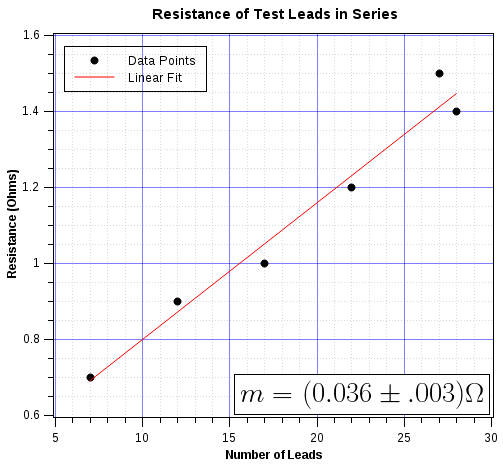
\includegraphics[width=\linewidth]{./lead_resistance.png}
  \caption{Linear fit used to obtain the average resistance of an individual lead.}
  \label{fig:lead_resistance}
  \end{center}
  \par\end{centering}
  \end{figure}

\textbf{Part 2}

\textit{Explain the observations made in items 3 and 4. What is the most important characteristic of a voltmeter, and why?}

The addition of a digital multi meter to the circuit caused nearly no difference in the circuit, due to its high resistance compared to the resistance of the circuit elements. However, the analog voltmeter, with a much lower resistance, exhibited a significant change in the circuit when it was wired parallel to the resistor and increased the current by over 24\%.
This is explained by the fact that adding resistive elements in parallel lowers the equivalent resistance, and from $V=iR$, increases the current if the voltage source is fixed.
Thus the effects of the voltmeter on the circuit becomes more pronounced at lower resistances, and the most important quality of a voltmeter is to have a resistance much higher than the elements being measured. \\

\textit{Explain any discrepancies in item 6 with voltage measured across the resistor using the multimeter. Does the ammeter affect the circuit? If so, how?}

When the ammeter was changed from the scale with a resistance of about 13 $\Omega$ to that of 5 $\Omega$, the voltage through $R_1$ increased by about 0.34\%. This follows from the fact that the ammeter was wired in series with the resistor, and had a small but nonzero resistance. Since the resistances added in series, the equivalent resistance of the circuit was increased, and the current was decreased slightly when the ammeter was added. This resulted in a slightly lower voltage across $R_1$, as the voltage drop was split over two resistive elements. This shows the importance of having an ammeter with as low of a resistance as possible, which would tend to minimize its effect on the rest of the circuit.

\textbf{Part 3}
\begin{enumerate}
 \item \textit{Series}: \begin{enumerate}
               \item \textit{Calculate the series equivalent resistance and compare it (with percent difference) to the measured value.}\\

		  From adding resistors in series, the theoretical equivalent resistance (according to the measured values) was equal to $(150.7 + 219.0 + 619) \Omega = 988.7 \Omega$.

		  This differs from the measured value of $988 \Omega$ by $0.071\%$. \\
               \item \textit{Verify Kirchoff's Voltage Rule by comparing the sum of the voltage drops across each of the resistors with the measured terminal voltage $V_T$.}\\

		  According to KVR,

		  $\Sigma V_{\text{loop}} =0 \Rightarrow $

		  $V_1 + V_2 + V_3  = V_s\Rightarrow $

		  $(0.783+1.141+3.223)\text{V} = 5.15\text{V}$ and

		  $5.147\text{V} \approx 5.15\text{V}$.

		  The percent error in the measured values was $0.0582\%$. \\

               \item \textit{Verify the voltage divider expression for one of the resistors, $V_{Ri} = V_S R_i / \sum R_i$}.\\

               Choosing $R_1$ shows that the theoretical voltage was

               $(5.15\text{V})(150.7\Omega)/(988\Omega) = .785\text{V}$.

               This differed from the measured voltage of $.783$V by $0.26\%$. \\
              \end{enumerate}

  \item \textit{Parallel}: \begin{enumerate}
                   \item \textit{Calculate the parallel equivalent resistance and compare it (with percent difference) to the measured value.}\\

                   Using the equation for adding resistors in parallel,

                   $1/R_{eq} = 1/R_1 + 1/R_2 \Rightarrow$

                   $R_{eq} = 162 \Omega$.

                   This differs from the measured resistance of $162.5 \Omega$ by $0.31\%$. \\

                   \item \textit{Verify Kirchoff's Current Rule by comparing the sum of the currents through the resistors with the measured current $I_s$.}\\

                   According to KCR, $\Sigma i_{\text{node} = 0}$. Summing the currents leaving the parallel branch,

                   $i_1 + i_2 = i_s \Rightarrow .02$A$+.01$A$ = .03$A,

                   which held true in this experiment.

                   However, due to possible equipment malfunctions, measurements on more precise scales were not able to be taken. Measuring these currents on the mA scale may have showed more deviation from the theoretical current.\\

                   \item \textit{Verify the current divider expression by calculating the current through one resistor and comparing it with the measured value, $I_{Ri} = I_S R_{eq} / R_i$.}\\

                   Choosing $R_1$, the current divider expression yields

                   $i_1 = i_s R_{eq} / R_1 \Rightarrow$

                   $i_1 = (.03$A$)(162.5 \Omega) / (620 \Omega) \Rightarrow$

                   $i_1 = .008$A, which differs from the measured current of .01 A by approximately $20\%$. Here, a more precise measurement may have yielded a value closer to the theoretical value.
                  \end{enumerate}


\end{enumerate}

\appendices{}

\section{Protoboard Diagram}\label{append:deriv}

\begin{figure}[h!]
  \begin{centering}
  \begin{center}
  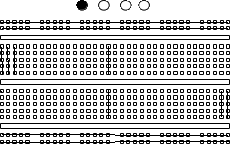
\includegraphics[width=\linewidth]{./proto.png}
  \label{fig:proto}
  \caption{General pattern of protoboard's internal wiring.}
  \end{center}
  \par\end{centering}
  \end{figure}

\section{Part 2 Circuit on Protoboard}

\begin{figure}[h!]
  \begin{centering}
  \begin{center}
  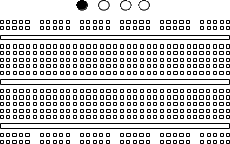
\includegraphics[width=\linewidth]{./proto_2.png}
  \label{fig:proto2}
  \caption{Schematic used to wire circuit in part 2.}
  \end{center}
  \par\end{centering}
  \end{figure}

%\bibliographystyle{plain}
%\bibliography{physbib}

\end{document}